%%%%%%%%%%%%%%%%%%%%%%%%%%%%%%%%%

\chapter{质点运动学}
%%%%%%%%%%%%%%%%%%%%%%%%%%%%%%%%%
质点运动学是研究质点运动规律的物理学分支,涉及质点的位移、速度、加速度等基本概念及其运动方程。

\marginnote[-17em]{
\indent
\key{质点:}忽略物体的形状和大小,只考虑物体的质量和位置的理想化物理模型。

\key{参考系:}观测者参考系或观察和描述物体运动的坐标系。

{\scriptsize \rmit{\quad 高中物理所谓参考系,通常是指观测者参考系中的惯性参考系。}}

\key{矢量:}既有大小又有方向的物理量

\key{标量:}只有大小没有方向的物理量。
}

%%%%%%%%%%%%%%%%%%%%%%%%%%%%%%%%%

\section{位矢,位移,速度,加速度}
%%%%%%%%%%%%%%%%%%%%%%%%%%%%%%%%%

\begin{marginfigure}[4.5cm]
    \includegraphics{/Position Vector/G-1/G1.pdf}
    \caption[Position vector]{
        位矢,位移,速度,加速度\\
        }
    \label{fig:Position Vector_G1}
\end{marginfigure}

\key{位矢:}位置矢量的简称,指从参考系原点指向质点位置的矢量。
记作$\symbfit{r}$,质点的运动就用位矢随时间的变化来描述,即
$$
\symbfit{r}= \symbfit{r}(t)
$$

\key{位移:}指物体在参考系中从初位置到末位置的有向线段。
记作$\Delta \symbfit{r}$,显然有
$$
\Delta \symbfit{r} = \symbfit{r}(t+\Delta t) - \symbfit{r}(t)
$$

{\small
高中人教版物理,位移常表示为$\Delta x$,为了叙事的方便,
后文将只在提起位矢时采用$\symbfit{r}$的写法,
而将$\Delta \symbfit{r}$简记为$x$,实际则为矢量。
}
\vspace{1em}

\key{速度:}指物体在单位时间内的位移量,即位矢的时间变化率。
记作$\symbfit{v}$,显然有
$$
\symbfit{v} = \lim_{\Delta t \to 0} \frac{\symbfit{r}(t+\Delta t) - \symbfit{r}(t)}{\Delta t}
= \lim_{\Delta t \to 0} \frac{\Delta \symbfit{r}}{\Delta t}
= \frac{\textup{d} \symbfit{r}}{\textup{d}t}
$$

\key{加速度:}指物体在单位时间内的速度变化量,即速度的时间变化率。记作$\symbfit{a}$,显然有
$$
\symbfit{a} = \lim_{\Delta t \to 0} \frac{\symbfit{v}(t+\Delta t) - \symbfit{v}(t)}{\Delta t}
= \lim_{\Delta t \to 0} \frac{\Delta \symbfit{v}}{\Delta t}
= \frac{\textup{d} \symbfit{v}}{\textup{d}t}
$$

%%%%%%%%%%%%%%%%%%%%%%%%%%%%%%%%%

\section{直角坐标系}
%%%%%%%%%%%%%%%%%%%%%%%%%%%%%%%%%
这里仅介绍直角坐标系及其变换,其他坐标系(如极坐标系、柱坐标系、球坐标系等)将在后续章节中介绍。
\begin{figure}
    \includegraphics[width=0.8\textwidth, keepaspectratio]{/Coordinate System/G-1/G1.pdf}
    \caption[Cartesian coordinate system]{
        直角坐标系\\
        \vspace{2cm}
        \normalsize
        基本矢量:${e}_x$,${e}_y$,${e}_z$
        }
    \label{fig:Coordinate System_G1}
\end{figure}

%%%%%%%%%%%%%%%%%%%%%%%%%%%%%%%%%

\section{常见运动类型}
%%%%%%%%%%%%%%%%%%%%%%%%%%%%%%%%%

\subsection{匀速直线运动}\marginnote{

$\symbfit{v}_0$:初始速度

$\symbfit{v}_t$:末速度
}

\subsection{匀变速直线运动}
\marginnote[2cm]{
    $$
    \begin{aligned}
        \symbfit{v}(t) &= \lim_{\Delta t \to 0} \frac{x}{\Delta t}\\
        &= \lim_{\Delta t \to 0} \frac{\symbfit{v}_0 (t_1 - t_2) + \frac{1}{2} \symbfit{a}(t_1^2 - t_2^2)}{t_1 - t_2}\\
        &= \lim_{\Delta t \to 0} \symbfit{v}_0 + \symbfit{a} \frac{t_1 + t_2}{2}\\
        &= \symbfit{v}_0 + \symbfit{a} t
    \end{aligned}
    $$
}
\begin{align*}
\symbfit{r}(t) &= \symbfit{v}_0 t + \frac{1}{2} \symbfit{a}t^2 = \frac{\symbfit{v}_0 + \symbfit{v}_t}{2} t \\
\Rightarrow x &= \symbfit{v}_0 (t_1 - t_2) + \frac{1}{2} \symbfit{a}(t_1^2 - t_2^2)\\
\\
\symbfit{v}(t) &= \symbfit{v}_0 + \symbfit{a} t\\
\Rightarrow \Delta \symbfit{v} &= \symbfit{a} \Delta t\\
\\
\symbfit{a}(t) &= \symbfit{a}
\end{align*}

速度位移关系:
$$
2\symbfit{a}x = \symbfit{v}_t^2 - \symbfit{v}_0^2
$$

中间时刻速度:
$$
\symbfit{v_\frac{t}{2}}(t) = \overline{\symbfit{v}} = \frac{(\symbfit{v}_0 + \symbfit{v} t)}{2}
$$

中间位置速度:
$$
\symbfit{v_\frac{\symbfit{r}}{2}}(t) = \sqrt{\frac{(\symbfit{v}_0^2 + \symbfit{v}_t^2)}{2}}
$$

\key{自由落体运动}

\subsection{斜抛运动}

\key{竖直上抛运动}

\key{平抛运动}

\key{竖直下抛运动}

\subsection{匀速率圆周运动}

{\small
注意,通常简称\textbf{“匀速率”}圆周运动为\textbf{“匀速”}圆周运动,实际并非匀速运动。
}
\vspace{1em}